\documentclass[12pt,a4paper]{article}
\usepackage{tikz}
\usetikzlibrary{trees}
\usepackage{amsmath}
\usepackage{forest}
\usepackage{commons/course}


%\hidesolutions



\شروع{نوشتار}
\سربرگ{}{آزمون پایان‌ترم}{25 خرداد ۱۳۹8}{}

\vspace*{-2in}
\begin{center}
	به نام او
\end{center}
\vspace*{1.5in}
- امتحان از 120 نمره می‌باشد و نمره کامل این امتحان، 90 می‌باشد.\\
- هر سوال را در یک صفحه جدا پاسخ دهید و مشخصات خود را در هر صفحه بنویسید.\\
- طراح سوالات: دکتر شریفی، علیرضا اکبری، شبنم شیخها، پدرام خورسندی، آراد محمدی، آریا کوثری، امیر مجتبی صبور و متین خواجوی\\
\vspace*{-0.5in}
\section*{سوالات کوتاه‌پاسخ (30 نمره)}
\شروع{ابجد}

\فقره درستی یا نادرستی عبارت زیر را مشخص کنید. جواب خود را توجیه کنید.(10نمره)
\شروع{فقرات}
\فقره یک آرایه‌ی $n$تایی از اعداد داریم که با ۱۰۰ عملِ جابجایی مرتب می‌شود. می‌توان الگوریتمی از $O(n)$ ارائه داد که این آرایه را مرتب کند. 
\فقره یک آرایه‌ی $n$تایی از اعداد طبیعی بین ۰ و 
$n ^ 2 - 1$
داریم. می‌توان الگوریتمی از $O(n)$ ارائه داد که این آرایه را مرتب کند.
\فقره اگر رأسی در د.د.ج دو فرزند داشته باشد، آن‌گاه عنصر بعدی آن فرزند راست، و عنصر قبلی آن فرزند چپ  ندارد. 
\فقره برای 
$n \geq 3$
عبارت "د.د.ج با $n$ گره که از طریق درج $n$ عدد با چینش تصادفی ساخته شده باشد" با عبارت "د.د.ج با $n$ گره که به تصادف و با احتمال مساوی از میان د.د.ج‌های با $n$ گره انتخاب شده باشد" از نظر مفهومی فرقی ندارد. 
\پایان{فقرات} 
\فقره یک گراف جهت‌دار به عنوان ورودی به ما داده شده است اما از بدون دور بودن آن اطلاعی نداریم. الگوریتم مرتب‌سازی توپولوژیک را به گونه‌ای اصلاح کنید که در صورتی که گراف بدون دور است، ترتیب توپولوژیک آن را بیابد و در غیر این صورت اعلام کند که گراف دور دارد. زمان اجرای این الگوریتم باید بر اساس اندازه‌ی ورودی خطی باشد

توجه کنید که تنها با اصلاح الگوریتم می‌بایست این کار را انجام دهید و نمی‌توانید از الگوریتم بخصوص یافتن دور در گراف استفاده کنید. همچنین اگر چند الگوریتم برای مرتب‌سازی توپولوژیک می‌شناسید، الگوریتم مناسب را تشخیص داده و آنرا اصلاح کنید.(10 نمره)

\فقره پیچیدگی زمانی هر یک از توابع زیر را بنویسید.(10 نمره)


\begin{flushleft}
	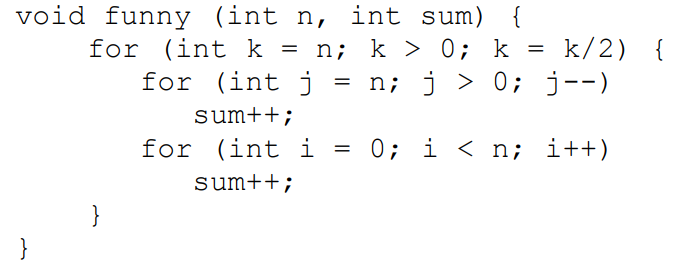
\includegraphics[]{figs/f1}
	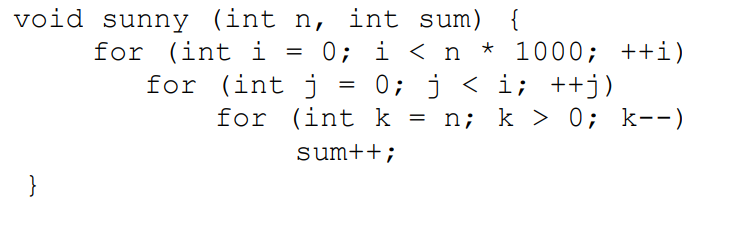
\includegraphics[]{figs/f2}
\end{flushleft}

\پایان{ابجد}

\newpage
\مسئله{مَمَّد در فینال لیگ قهرمانان اروپا(20 نمره)}
ممّد از سری دانشجوهایی است که به لباس هایش بسیار اهمیت می‌دهد و حوصله متین را همیشه با لباس‌ها و وسواس انتخاب لباس، سر می‌برد. وسواسش به حدی است که او تمام لباس های خود را بر اساس میزان علاقه‌اش به این لباس‌ها در کمدش و به صورت یک جدول $m*n$ مرتب کرده است. خاصیت این جدول این است که هر سطر از چپ به راست و هر ستون از بالا به پایین به صورت صعودی مرتب شده است. بعضی از نقاط این جدول می‌تواند $\infty$ باشد که به معنی عدم وجود لباسی در آن‌خانه است. (توجه کنید که مقدار $\infty$ از اعداد موجود در جدول بزرگتر است.) در زیر یک مثال از یک کمد $4*4$ آمده است:
\begin{center}
	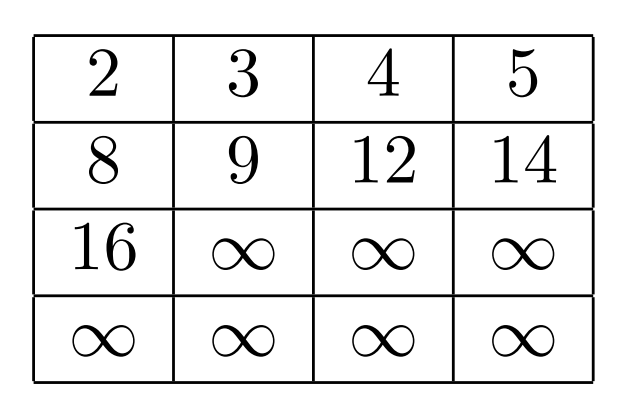
\includegraphics[width=1.3in, height=1.2in]{figs/table}
\end{center}
به تازگی به دلیل زیاد بودن لباس‌ها ممد به مشکل خورده است و می‌خواهد تا برای کمدش سیستمی تعریف کند تا:


-	بی ارزش ترین لباس کمد را از کمد خارج کند. (تضمین می‌شود جدول خالی نیست.)(10 نمره)\\
-	یک لباس جدید را در کمد درج کند. (تضمین می‌شود جدول پر نیست.)(5 نمره)\\
-	فقط با استفاده از حافظه‌ی اضافی $O(1)$، فهرست مرتب‌شده‌ی لباس‌های قرار گرفته در یک جدول $n \times n$ را چاپ کند. توجه کنید وضعیت جدول بعد از اجرای الگوریتم به انتخاب شماست.(5 نمره)


ممد برای حل این مشکل در هفته قبل از فینال لیگ قهرمانان اروپا به متین مراجعه می‌کند و متین تنها به شرطی که ممد قول دهد با یکی از لباس‌های زیبایش به وسط مسابقه فینال برود قبول می‌کند تا مشکل او را حل کند. 


متین 3 سوال را حل کرد و حال از شما نیز می‌خواهد حل کنید.\\
پیچیدگی زمانی دو بخش اول باید $O(m+n)$ باشد و خاصیت مرتب بودن جدول بعد از انجام هر عملیات حفظ شود. پیچیدگی زمانی بخش سوم $O(n^3)$ است. در هر بخش ثابت کنید پیچیدگی زمانی الگوریتم شما همان پیچیدگی زمانی خواسته شده است.\\
\\


\مسئله{واسه همه پیگیری‌هات مرسی(15 نمره)}
اکبر سلطانِ چندین ویلا در کُردان می‌باشد. وی که برای طراحی امتحان پایان‌ترم می‌بایست به متین کمک می‌کرد، پیگیری‌های زیادی از او بابت امتحان انجام داد و متین از آنجایی که یک جنتلمن واقعی است، برای تشکر از پیگیری‌های اکبر، می‌خواهد به او در یکی از مشکلاتش کمک کند.


نقشه‌ی کَردان یک گراف بدون جهت هم‌بند هست که راس‌های آن‌ ویلاهای اکبر هستند و هر یال آن یک کوچه است که دو ویلا را به هم متصل می‌کند.(فرض نکنید گراف مسطح است، یعنی کوچه‌ها می‌توانند با پل یا تونل از هم عبور کنند) حال او با شروع از یک ویلای دلخواه  $v$ الگوریتم جستجوی سطح اول\lr{(BFS)} اجرا کرده است و درخت پوشایی که در نتیجه اجرای این الگوریتم به دست می‌آید را 
$T_1$
نامیده است.همچنین بار دیگر با شروع از ویلای 
$v$
الگوریتم جستجوی عمق اول\lr{(DFS)} را اجرا کرده است و درخت پوشایی که این بار بدست می‌آید را 
$T_2$
نامیده‌ است. 

به اکبر کمک کنید ثابت کند که  
$T_1$
و 
$T_2$
با هم برابر هستند(یعنی مجموعه‌ی یال‌های برابری دارند) اگر و تنها اگر نقشه کُردان خود یک درخت باشد. 
\\

\newpage
\مسئله {مسیریابی(15 نمره)}
در یک شهر $n$ تقاطع (میدان، چهارراه یا هر نوع تقاطع دیگر) که با شماره‌های ۱ تا $n$ شماره‌گذاری شده‌اند، و $m$ خیابان که با شماره‌های ۱ تا $m$ شماره‌گذاری شده‌اند وجود دارد. 
خیابان $i$ ام، تقاطع‌های با شماره‌ی $A_i$ و $B_i$ را به صورت دوطرفه به یک‌دیگر متصل می‌کند. هر تقاطع ممکن است به یک یا تعداد دل‌خواهی خیابان متصل باشد. در این شهر، می‌توان با عبور از خیابان‌ها بین هر دو تقاطع دلخواهی سفر کرد.

شما یک اپ مسیریابی توسعه داده‌اید. در این اپ، یک راننده دو تقاطع مبدا و مقصد را مشخص می‌کند و شما می‌بایست سریع‌ترین مسیر برای رسیدن به مقصد را مشخص کنید. برای سادگی کار، فرض کنید ترافیک خیابان‌ها و تقاطع‌ها در طول پیمودن مسیر ثابت است.
بر اساس اطلاعات دریافتی از همه‌ی رانندگان،  زمان پیمودن هر خیابان و تقاطع را تخمین زده‌‌اید. به طور دقیق‌تر، پیمودن خیابان $i$ ام از یک انتها به انتهای دیگر آن به اندازه‌ی $S_i$ ثانیه طول می‌کشد و تفاوتی ندارد که خیابان را در کدام جهت طی کنید. 
هم‌چنین وقتی در مسیر  به یک تقاطع $j$ می‌رسیم، باید مدت زمان $T_j$ ثانیه در آن تقاطع صبر کنیم (مثلا متوسط زمان انتظار پشت چراغ قرمز). این موضوع برای تقاطع‌های مبدا و مقصد صادق نیست. تمام مقادیر $S_i$ و $T_j$ نامنفی است.

برای هر یک از دو حالت زیر، الگوریتم کارآمدی پیشنهاد دهید که با گرفتن اطلاعات شهر و یک مبدا و مقصد مشخص، کوتاه‌ترین مسیر بین مبدا و مقصد و زمان پیمودن مسیر را مشخص کند. اگر پاسخ شما برای حالت دوم درست باشد، نیازی به حل حالت اول نیست.
\شروع {ابجد}
\فقره اگر همه‌ی $S_i$ برابر ۱ و همه‌ی مقادیر $T_i$ برابر صفر باشد.(5 نمره)
\فقره در حالت کلی.(10 نمره)
\پایان {ابجد}

\مسئله{پیش از تابستان\footnote{به تقلید از سه‌گانه "پیش از" اثر ریچارد لینکلیتر}(20 نمره)}

سال پیش متین در هواپیمای مشهد به تهران بود که دکتر شریفی را دید و ناگهان تصمیم گرفت تا دستیار آموزشی شود. او خود را به دکتر معرفی کرد و به ایشان گفت که در تابستان به سفری طولانی خواهد رفت اما تا آن زمان می‌خواهد به ایشان در تیم تدریس دروس ارائه‌شده توسط ایشان کمک کند. دکتر با موافقت یکساله، درخواست او را مبنی بر دستیار آموزشی شدن قبول کرد و همکاری او با دکتر شروع شد. 


حال زمان یکساله رو به پایان است و در این مدت متین متوجه شده است که دوست دارد برای زمان بیشتری دستیار ایشان باشد و علاقه زیادی به این کار پیدا کرده‌ است، اما به دلیل نزدیکی تابستان و سفر پیش رو چاره‌ای جز خداحافظی نمی‌بیند.


دکتر شریفی رشته‌ای به طول $n$ را به او به عنوان یادگاری می‌دهد. این رشته شامل یک معما می‌باشد که با حل آن متین می‌تواند دوباره دستیار آموزشی شود. این معما به این صورت است که در این رشته، باید بزرگترین زیر رشته‌ای را بیابد که هم پیشوند، هم میانوند و هم پسوند باشد. 


به متین کمک کنید تا در زمان $O(n)$ معما را حل کند. (میان‌وندِ یک رشته، یک زیررشته از آن است که شامل حرف اول و آخر رشته‌ی اصلی نباشد.)

\newpage
\مسئله{سَم(20 نمره)}
در طی مسیر دانشگاه تا خانه دکتر شریفی یک تالاب وجود دارد که ایشان را وادار میکند برای رفتن به دانشگاه، از این تالاب عبور کند. این تالاب با یک مربع به ضلع 
$n$ 
توصیف میشود.
\\
درون این دریاچه ماری سمی زندگی میکند. این مار به شکل مسیری که هر راس از آن دقیقا یک خانه از جدول 
$n \times n$ 
تالاب را پر میکند توصیف شده است. دم مار خارج از دریاچه قرار دارد و در صورت برخورد دکتر شریفی با سر مار، مار دکتر شریفی را نیش میزند. در زیر یک مثال از تالابی با $n=3$ آمده است.
\begin{figure}[h!]
	\centering
	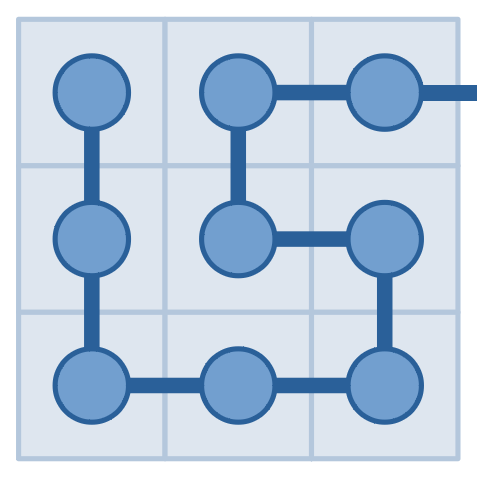
\includegraphics[width=1.7in, height=1.7in]{figs/mar}
	\caption{سر مار در خانه $[1,1]$ قرار دارد و دم آن از خانه $[1,3]$ خارج شده است.}
\end{figure}
\\
برای یافتن سر مار، دستگاهی در اختیار دکتر شریفی قرار دارد. این دستگاه با دریافت یک مستطیل از تالاب تعداد دفعاتی که مار با مرز‌های مستطیل برخورد داشته را نشان می‌دهد. در شکل زیر یک مثال از زیر مستطیل مشخص شده توسط دکتر را مشاهده می‌کنید. دستگاه در پاسخ عدد ۴ را نشان می‌دهد که در شکل با ستاره مشخص شده است.
\\
\begin{figure}[h!]
	\centering
	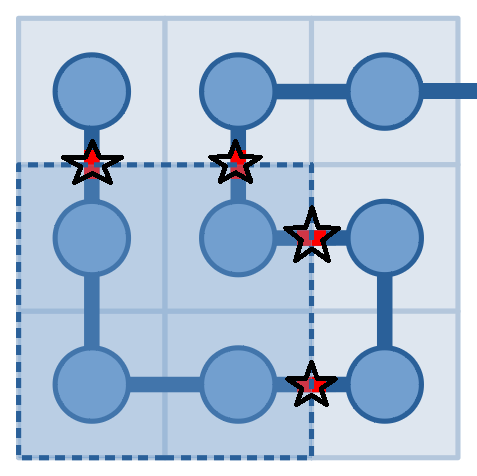
\includegraphics[width=1.7in, height=1.7in]{figs/mar1}
	\caption{جوابی که دکتر می‌گیرد 4 است.}
\end{figure}
\\
الگوریتمی ارائه دهید که با  
$O(lg~n)$ 
بار استفاده از دستگاه سر مار را بیابد.

\پایان{نوشتار}
